\begin{tiny}Eig08\end{tiny} Intégrale de Dirichlet.\newline
\begin{figure}[h!]
 \centering
 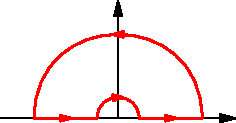
\includegraphics{./Eig08_1.pdf}
 % Eig08_1.pdf: 113x59 pixel, 72dpi, 3.99x2.08 cm, bb=0 0 113 59
 \caption{Exercice \arabic{enumi}}
 \label{fig:Eig08_1}
\end{figure}
Soit $\mathcal{D}$ l'ensemble des points $m$ d'un plan rapporté à un repère tels que $|x(m)|+y(m)>0$. On définit les fonctions $A$ et $B$ par
\begin{align*}
 &A= \frac{e^{-y}}{x^2+y^2}\left( x\sin x - y\cos x\right) \\
 &B= \frac{e^{-y}}{x^2+y^2}\left( x\cos x + y\sin x\right)
\end{align*}
On note $\omega = Adx +Bdy$ et
\begin{displaymath}
 I(r) = \int_0^\pi e^{-r\sin \theta}\cos(r\cos\theta)d\theta
\end{displaymath}
et on admet que $I \xrightarrow{+\infty}0$ et $I \xrightarrow{0}\pi$.
\begin{enumerate}
 \item Dessiner le domaine $\mathcal{D}$. Est-il étoilé ?
 \item Calculer $\frac{\partial A}{\partial y}$ et $\frac{\partial B}{\partial x}$.
 \item Montrer que l'intégrale curviligne de $\omega$ le long de la courbe constituée de segments et de demi-cercles (de rayon $0<r<R$ (figure \ref{fig:Eig08_1}) est nulle.
 \item En exprimant cette intégrale curviligne d'une autre manière montrer que, quand $r\rightarrow 0$,
\begin{displaymath}
 \int_r^{\frac{1}{r}}\frac{\sin t}{t}dt \rightarrow \frac{\pi}{2}
\end{displaymath}

\end{enumerate}
